\documentclass[class=book, crop=false, oneside]{standalone}
\usepackage[subpreambles=true]{standalone}

\usepackage{../../style}

\graphicspath{{./assets/images/}}
% arara: pdflatex: { synctex: yes, shell: yes }
% arara: latexmk: { clean: partial }
\begin{document}
\chapter{Proprietà dei linguaggi context free}

\section{Proprietà di chiusura}

\subsection*{Chiusura rispetto all'unione}
\begin{lemma}
  La classe dei linguaggi liberi è chiusa rispetto all'operazione di unione d'insiemi.
  \begin{equation*}
    \textrm{Se } \mathcal{L}_1 \land \mathcal{L}_2 \textrm{ sono liberi} \implies \mathcal{L}_1 \cup \mathcal{L}_2 \textrm{ è libero}
  \end{equation*}
\end{lemma}

\begin{proof}
    Siano \(\mathcal{L}_1\) e \(\mathcal{L}_2\) dei linguaggi liberi; questo vuol dire che devono esistere due grammatiche libere, ciascuna delle quali ha generato uno dei due linguaggi. In simboli:

  \begin{equation*}
    \exists \mathcal{G}_1 = (V_1, T_1, S_1, \mathcal{P}_1), \mathcal{G}_2 = (V_2, T_2, S_2, \mathcal{P}_2) : \mathcal{L}_1 = \mathcal{L}(\mathcal{G}_1) \textrm{ e } \mathcal{L}_2 = \mathcal{L}(\mathcal{G}_2)
  \end{equation*}

  Vediamo quindi come costruire una nuova grammatica libera che possa generare l'unione dei due linguaggi generati dalle rispettive grammatiche viste sopra. Consideriamo quindi una nuova grammatica \(\mathcal{G}\), i cui elementi sono così definiti:

  \begin{equation*}
      \mathcal{G} = (V'_1 \cup V'_2 \cup \{S\}, T_1 \cup T_2, S, \mathcal{P}'_1 \cup \mathcal{P}'_2 \cup \{S \rightarrow S'_1 | S'_2\})
  \end{equation*}

  \noindent Andiamo a vedere da vicino come sono stati ricavati gli elementi:

  \begin{itemize}
    \item \(V'_1\) e \(V'_2\) si ottengo effettuando un'operazione di \emph{refresh} sui non terminali, in modo da evitare collisioni di nomi (vedremo più avanti come mai quest'operazione è importante), inoltre questo vocabolario è completato con l'introduzione di un nuovo starting symbol;
    \item l'insieme dei terminali è l'unione dei sue insiemi di terminali di \(\mathcal{G}_1\) e \(\mathcal{G}_2\);
    \item \(S\) è il nuovo starting symbol, non presente in \((V'_1 \cup V'_2\), e \(S'_1\) e \(S'_2\) sono di nuovo il refresh degli starting symbol rispettivamente di \(\mathcal{G}_2\) e \(\mathcal{G}_2\);
    \item infine, l'insieme delle produzioni è dato dall'unione tra i refresh delle produzioni delle due grammatiche di partenza  \(\mathcal{G}_1\) e \(\mathcal{G}_2\), unito a una nuova produzione che, dal nuovo starting symbol, produce il resfresh dello starting symbol di una delle due grammatiche di partenza.
  \end{itemize}

  \noindent Questa definizione ci basta per asserire che \(\mathcal{L(G)}\) è libero e \(\mathcal{L(G)} = \mathcal{L(G)_1} \cup \mathcal{L(G)_2}\).

\end{proof}

\begin{osservazione}
  Cerchiamo di capire come mai possiamo essere certi che la grammatica \(\mathcal{G}\), per come l'abbiamo definita, è libera.

  Prendiamo l'insieme delle produzioni di \(\mathcal{G}\); abbiamo già visto come è stato ricavato. Il refreshing va a colpire solamente i nomi dei terminali o non-terminali, non la loro forma, che rimane immutata (\(A \implies \alpha\)). Questa forma è rispettata anche dalle due nuove produzioni aggiunte (\(S \implies S'_1\) e \(S \implies S'_2\)) (e tipo quindi?)

\end{osservazione}

\begin{osservazione}
  Cerchiamo di capire come mai  \(\mathcal{L(G)} = \mathcal{L(G)_1} \cup \mathcal{L(G)_2}\) è valido.
  \begin{itemize}
    \item Consideriamo una stringa \(w \in \mathcal{L(G)}\); questo è vero se e solo se esiste una certa derivazione per ottenerla a partire dallo starting symbol (\(S \implies^* w\)).
    \item Per come abbiamo definito la grammatica \(\mathcal{G}\), il secondo passo della derivazione dev'essere necessariamente il refresh di uno dei due starting symbol delle grammatiche di partenza (\(S \implies S'_1 \implies^* w \lor S \implies S'_2 \implies^* w\));
    \item questo naturalmente è valido se e solo se, a questo punto, la stringa \(w\) può essere derivata in qualche modo a partire da uno degli starting symbol delle grammatiche di partenza (\(S_1 \implies^* w \lor S_2 \implies^* w\)).
    \item Se \(w\) può essere ottenuta attraverso qualche derivazione a partire da \(S_1\) o \(S_2\), allora vuol dire che \(w\) appartiene a uno dei due linguaggi generati dalle nostre due grammatiche di partenza (\(w \in \mathcal{L(G)}_1 \lor w \in \mathcal{L(G)}_2\)).
    \item Questo è equivalente ad affermare che \(w\) appartiene all'unione dei due linguaggi (\(w \in \mathcal{L(G)}_1 \cup \mathcal{L(G)}_2\)), e ci convince quindi della validità dell'asserto.
  \end{itemize}
\end{osservazione}

\begin{osservazione}
  È semplice convincersi dell'importanza dell'operazione di refreshing. Se consideriamo due grammatiche \(\mathcal{G}_1, \mathcal{G}_2\) con le seguenti produzioni:
  \begin{figure}
    \centering
    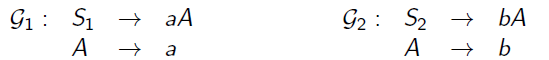
\includegraphics[width=.7\textwidth,keepaspectratio]{prod-g1-g2}
  \end{figure}
  \noindent Avremo quindi generati i seguenti linguaggi: \(\mathcal{L(G)}_1 = \{aa\}\) e \(\mathcal{L(G)}_2 = \{bb\}\).

  Se non effettuassimo refreshing, Ci troveremo ad avere una nuova grammatica con le seguenti produzioni:
  \begin{figure}
    \centering
    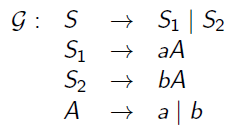
\includegraphics[width=.3\textwidth,keepaspectratio]{prod-g-naive}
  \end{figure}
  \noindent Il linguaggio prodotto da questa nuova grammatica sarebbe diverso da quello dato dall'unione delle due grammatiche di partenza, poiché avremmo \(\mathcal{L(G)} = \{aa, ab, ba, bb\} \neq mathcal{L(G)}_1 \cup \mathcal{L(G)}_2\).

  Con un'opportuno resfreshing otteniamo invece:
  \begin{figure}
    \centering
    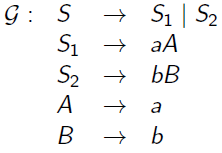
\includegraphics[width=.3\textwidth,keepaspectratio]{prod-g}
  \end{figure}
  Questo insieme di produzioni garantisce che la grammatica generi il linguaggio desiderato.
\end{osservazione}

\subsection*{Chiusura rispetto alla concatenazione}

\begin{lemma}
  La classe dei linguaggi liberi è chiusa rispetto all'operazione di concatenazione.

  \begin{equation*}
    \textrm{Se } \mathcal{L}_1 \land \mathcal{L}_2 \textrm{ sono liberi} \implies \{w_1w_2 | w_1 \in \mathcal{L}_1 \land w_2 \in \mathcal{L}_2\} \textrm{ è un linguaggio libero.}
  \end{equation*}

\end{lemma}

\begin{proof}
  % Consideriamo due linguaggi liberi \(\mathcal{L}_1\) e \(\mathcal{L}_2\);
  La dimostrazione sembra assolutamente uguale a quella del lemma della chiusura all'unione, sono confuso ma domani cercherò di chiarire.
\end{proof}


\section{Chomsky Normal Form}
\paragraph{Definizione}
Una grammatica libera \(\mathcal{G} = (V, T, S, \mathcal{P})\) è in \emph{Chomsky Normal Form} se e solo se:
\begin{itemize}
  \item non ha alcuna \(\epsilon\)-produzione, al massimo \(S \implies \epsilon\);
  \item tutte le sue non \(\epsilon\)-produzioni  una tra le due seguenti forme:
  \begin{itemize}
    \item \(A \implies a\)
    \item \(A \implies BC\)
  \end{itemize}
  in cui sia \(B\) sia \(C\) sono diversi da \(S\).
\end{itemize}

\begin{lemma}
  Sia \(\mathcal{G}\) una grammatica libera; allora esiste una certa grammatica \(\mathcal{G'}\) in Chomsky Normal Form tale che \(\mathcal{L(G)} = \mathcal{L(G')}\).
\end{lemma}

\noindent La dimostrazione del lemma è lasciata per esercizio.


\section{Pumping lemma for free languages}

\end{document}
